\documentclass[a4paper, 12pt]{article}
\usepackage[bottom=5em, top=5em]{geometry}
\usepackage{color}
\usepackage{graphicx}
\usepackage{verbatim}
\begin{document}

\title{Deep Learning Lab Report \\ Assignment 3}
\author{Ravin Kohli}
\maketitle

\section{Objective}
\textbf{Training Encoder-Decoder network with 4 different configurations of the decoder network}\\
We were tasked with training an encoder-decoder network for semantic segmentation. The main aim of the task is to analyse the impact of the number of upsamples performed on the performance of the network. We implemented four configurations 
\begin{enumerate}
	\item Single Upsample -16x (hereby referred to as Configuration 1)
	\item Two Upsamples -2x $\rightarrow$ 8x (hereby referred to as Configuration 2)
	\item Three Upsamples -2x $\rightarrow$ 2x $\rightarrow$ 4x (hereby referred to as Configuration 3)
	\item Four Upsamples -2x $\rightarrow$2x$\rightarrow$2x $\rightarrow$ 2x (hereby referred to as Configuration4)
\end{enumerate}

\section{Network Architecture}
Architecture of the Decoder Network
\begin{enumerate}
	\item Configuration 1 - There is no refinement block and we directly upsample the feature map from the encoder to the size of the image.
		\begin{table}[h]
			\caption{Configuration 1}
			\begin{tabular}{|l|l|l|l|}
				\hline
				\textbf{Layer Number} & \textbf{Output Feature maps} & \textbf{Upsampling Rate} & \textbf{Kernel size} \\
				%heading
				\hline
				Upsample 1 & 120 & 16 & 3\\
				\hline
				Conv & No. of Classes & 1 & 1\\
				\hline
			\end{tabular}
		\end{table}
	\item Configuration 2 - There is one refinement block with its corresponding skip connection.
	\begin{figure}[h]
		\centering
		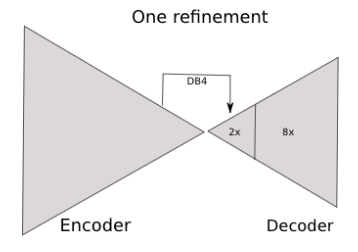
\includegraphics[height= 0.1\textheight]{onerefinement}
		\label{image1-onerefinement}
	\end{figure}
	\begin{table}[h]
		\caption{Configuration 2}
		\begin{tabular}{|l|l|l|l|}
			\hline
			\textbf{Layer Number} & \textbf{Output Feature maps} & \textbf{Upsampling Rate} & \textbf{Kernel size} \\
			%heading
			\hline
			Upsample 1 & 256 & 2 & 3\\
			\hline
			Conv 1& 256 & 1 & 3\\
			\hline
			Upsample 2& 120 & 8 & 3\\
			\hline
			Conv 2& No. of Classes & 1 & 1\\
			\hline
		\end{tabular}
	\end{table}
\newpage
\item Configuration 3 - There are two refinement blocks with their corresponding skip connections.
\begin{figure}[h]
	\centering
	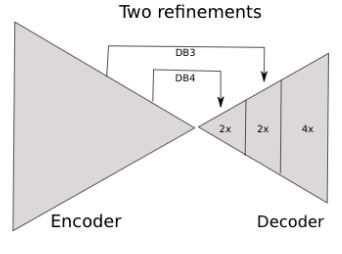
\includegraphics[height= 0.1\textheight]{tworefinement}
	\label{image2-tworefinement}
\end{figure}
\begin{table}[h]
	\caption{Configuration 3}
	\begin{tabular}{|l|l|l|l|}
		\hline
		\textbf{Layer Number} & \textbf{Output Feature maps} & \textbf{Upsampling Rate} & \textbf{Kernel size} \\
		%heading
		\hline
		Upsample 1 & 256 & 2 & 3\\
		\hline
		Conv 1& 256 & 1 & 3\\
		\hline
		Upsample 2& 160 & 2 & 3\\
		\hline
		Conv 2& 160 & 1 & 1\\
		\hline
		Upsample 3& 120 & 4 & 3\\
		\hline
		Conv 3& No. of Classes & 1 & 1\\
		\hline
	\end{tabular}
\end{table}
\item Configuration 4 - There are three refinement blocks with their corresponding skip connections.
\begin{figure}[h!]
	\centering
	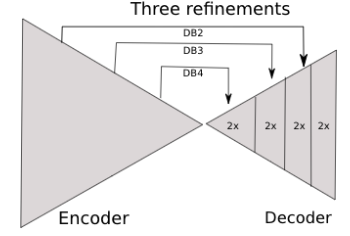
\includegraphics[height= 0.1\textheight]{threerefinement}
	\label{image3-threerefinement}
\end{figure}
\newpage
\begin{table}[h]
	\caption{Configuration 4}
	\begin{tabular}{|l|l|l|l|}
		\hline
		\textbf{Layer Number} & \textbf{Output Feature maps} & \textbf{Upsampling Rate} & \textbf{Kernel size} \\
		%heading
		\hline
		Upsample 1 & 256 & 2 & 3\\
		\hline
		Conv 1& 256 & 1 & 3\\
		\hline
		Upsample 2& 160 & 2 & 3\\
		\hline
		Conv 2& 160 & 1 & 1\\
		\hline
		Upsample 3& 96 & 2 & 3\\
		\hline
		Conv 3& 96 & 1 & 3\\
		\hline
		Upsample 4& 120 & 4 & 3\\
		\hline
		Conv 4& No. of Classes & 1 & 1\\
		\hline
	\end{tabular}
\end{table}
\end{enumerate}
\section{Results}
\begin{figure}[h!]
	\centering
	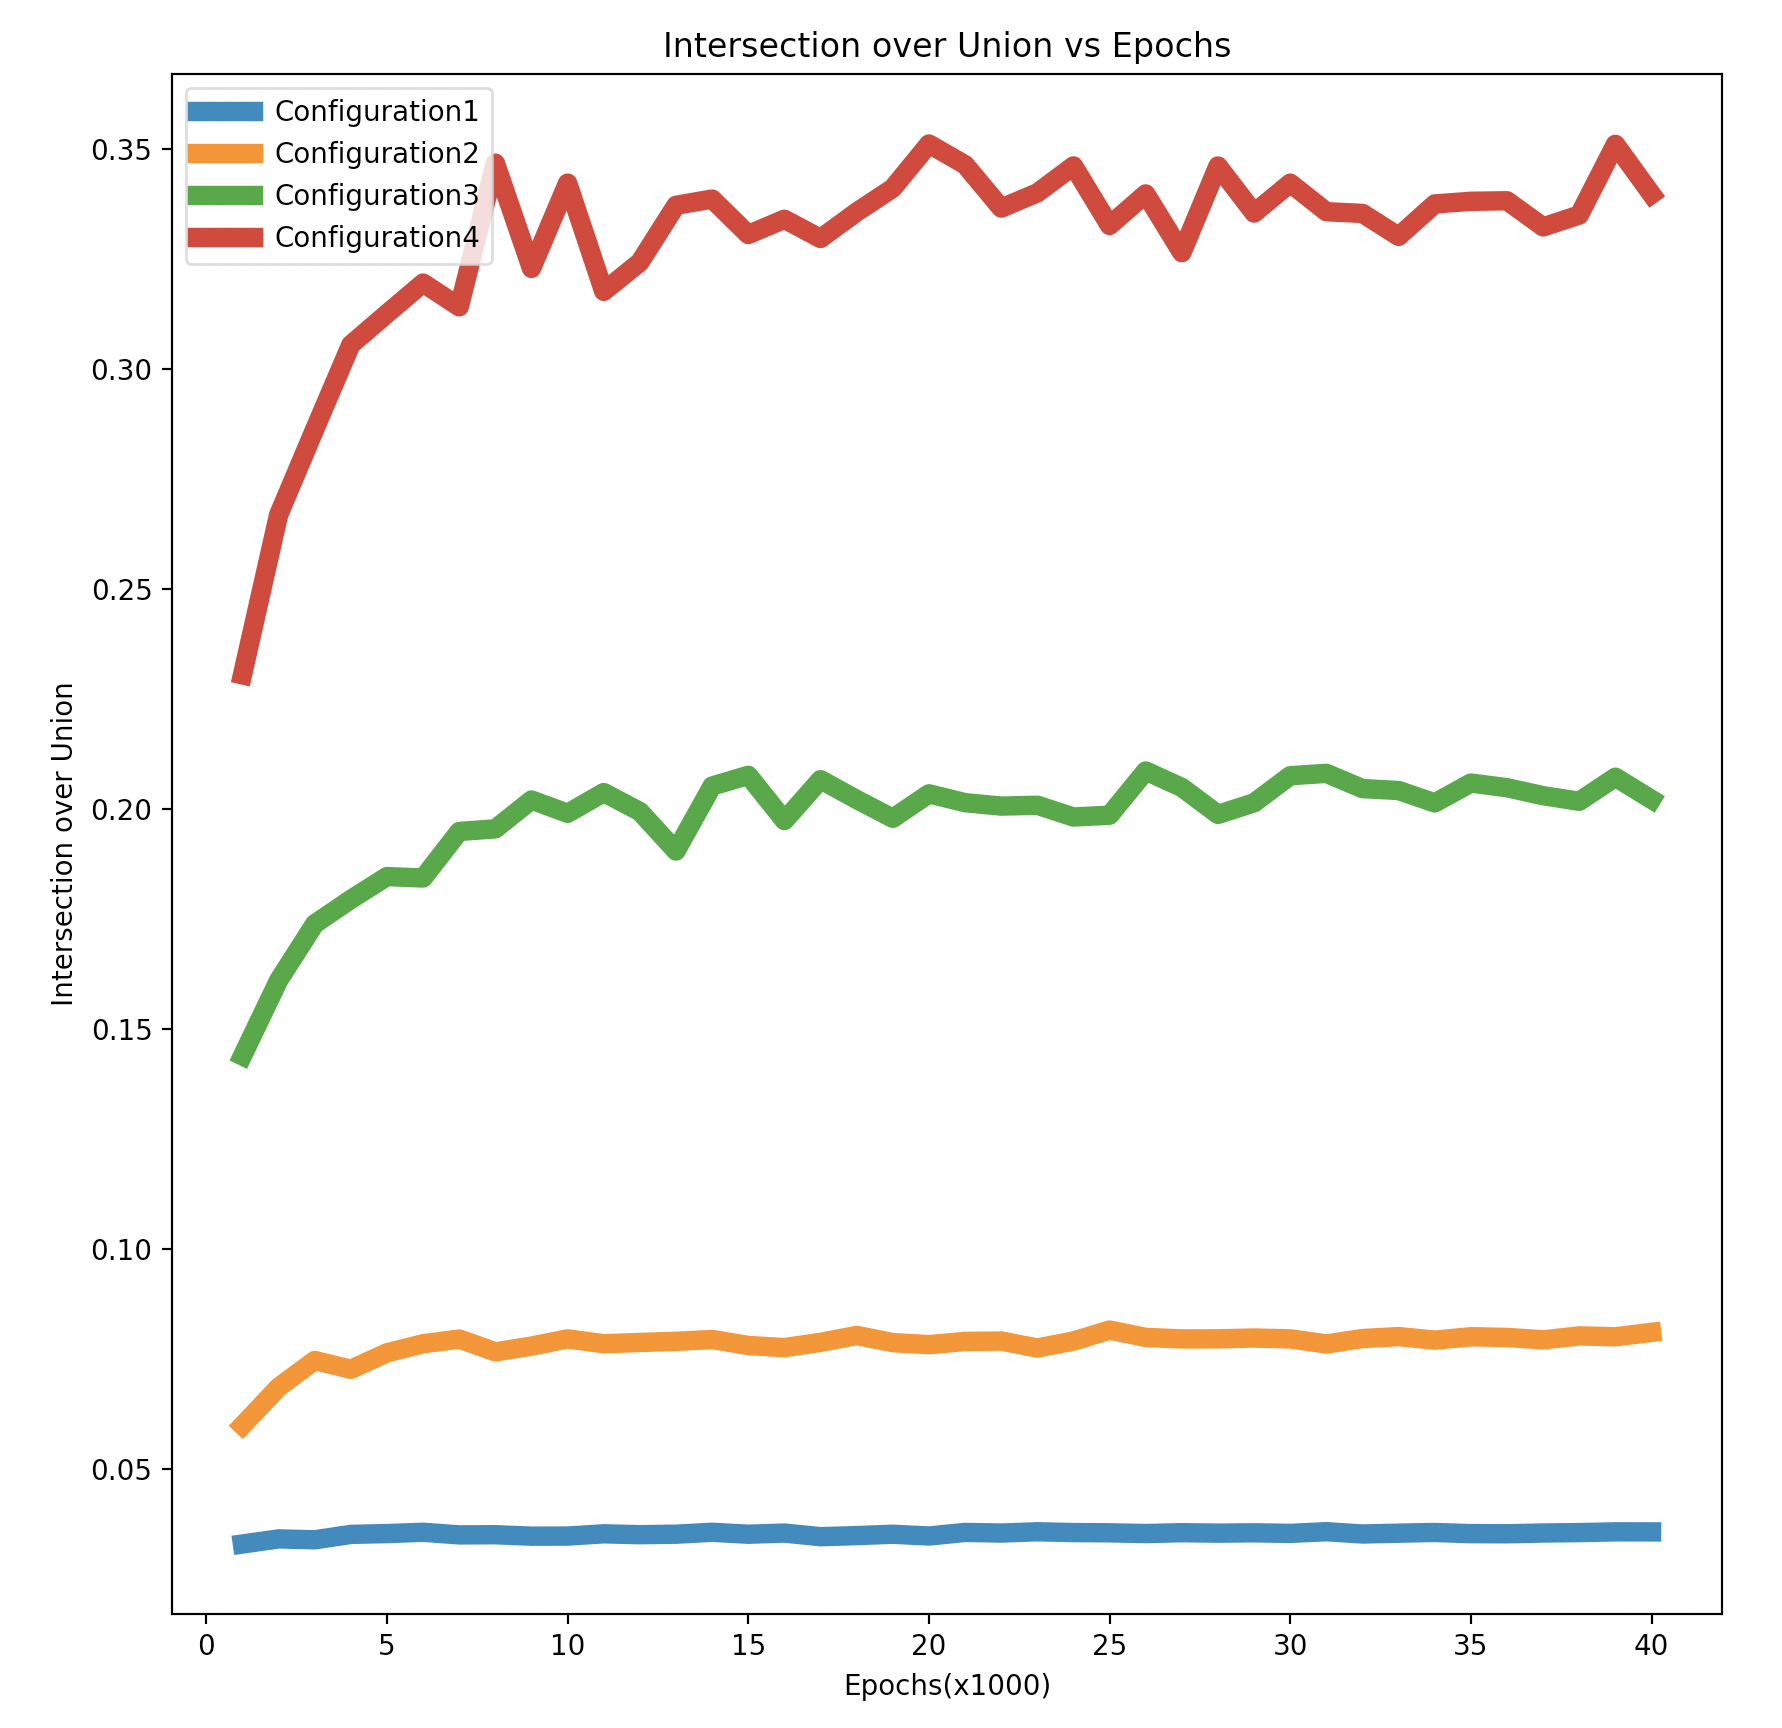
\includegraphics[width=0.7\linewidth, height=0.32\textheight]{iouvsepoch}
	\label{image4-iouvsepoch}
	\caption{IoU vs Epochs}
\end{figure}
\begin{table}[h]
	\caption{Results}
	\centering
	\begin{tabular}{|l|l|}
		\hline
		\textbf{Configuration} & \textbf{IoU} \\
		%heading
		\hline
		Configuration 1 & 0.035\\
		\hline
		Configuration 2& 0.081\\
		\hline
		Configuration 3& 0.202\\
		\hline
		Configuration 4& 0.339\\
		\hline
	\end{tabular}
\end{table}
\newpage
\section{Conclusion}
We have tested four configurations according to the number of refinement blocks present in them. The best performing configuration is with using three refinement blocks and upsampling it 2x in every step. This can be understood as increasing the number of upsampling increases the number of parameters to be learnt. Also, this configuration has 3 skip connections. That means it is using the output from the convolutional layers in the encoder part of the network and feeding it into the output of the upsampling which in turn helps the network to estimate the image well.
\end{document}